\documentclass[twoside,twocolumn, elsart]{article}

\usepackage{blindtext} % Package to generate dummy text throughout this template 

\usepackage[sc]{mathpazo} % Use the Palatino font
\usepackage[T1]{fontenc} % Use 8-bit encoding that has 256 glyphs
\linespread{1.05} % Line spacing - Palatino needs more space between lines
\usepackage{microtype} % Slightly tweak font spacing for aesthetics

\usepackage[english]{babel} % Language hyphenation and typographical rules

\usepackage[hmarginratio=1:1,top=32mm,columnsep=20pt]{geometry} % Document margins
\usepackage[hang, small,labelfont=bf,up,textfont=it,up]{caption} % Custom captions under/above floats in tables or figures
\usepackage{booktabs} % Horizontal rules in tables

\usepackage{lettrine} % The lettrine is the first enlarged letter at the beginning of the text

\usepackage{enumitem} % Customized lists
\setlist[itemize]{noitemsep} % Make itemize lists more compact

\usepackage{abstract} % Allows abstract customization
\renewcommand{\abstractnamefont}{\normalfont\bfseries} % Set the "Abstract" text to bold
\renewcommand{\abstracttextfont}{\normalfont\small\itshape} % Set the abstract itself to small italic text

\usepackage{titlesec} % Allows customization of titles
\renewcommand\thesection{\Roman{section}} % Roman numerals for the sections
\renewcommand\thesubsection{\roman{subsection}} % roman numerals for subsections
\titleformat{\section}[block]{\large\scshape\centering}{\thesection.}{1em}{} % Change the look of the section titles
\titleformat{\subsection}[block]{\large}{\thesubsection.}{1em}{} % Change the look of the section titles

\usepackage{fancyhdr} % Headers and footers
\pagestyle{fancy} % All pages have headers and footers
\fancyhead{} % Blank out the default header
\fancyfoot{} % Blank out the default footer
\fancyhead[C]{Running title $\bullet$ May 2016 $\bullet$ Vol. XXI, No. 1} % Custom header text
\fancyfoot[RO,LE]{\thepage} % Custom footer text

\usepackage{titling} % Customizing the title section

\usepackage{hyperref} % For hyperlinks in the PDF
\usepackage{ulem}
\usepackage[usenames]{color}
\usepackage{epsfig}
\usepackage{graphicx}
\usepackage{times}
\usepackage{dcolumn}
\usepackage{slashbox,pict2e}
\usepackage{polski}

%\newcommand{\vec}[1]{\boldsymbol{#1}}
%\newcommand{\angstrom}{\textup{\AA}}



%----------------------------------------------------------------------------------------
%	TITLE SECTION
%----------------------------------------------------------------------------------------

\setlength{\droptitle}{-4\baselineskip} % Move the title up

\pretitle{\begin{center}\Huge\bfseries} % Article title formatting
\posttitle{\end{center}} % Article title closing formatting
\title{Resonant Inelastic X-ray Spectroscopy on $LiCu_3 O_3$ } 
\author{%
\textsc{R. Świętek}\thanks{A thank you or further information} \\[1ex] 
\normalsize Wrocław University of Science and Technology, Wrocław 50-370, Poland \\ 
%\normalsize \href{mailto:john@smith.com} % Your email address
%\and % Uncomment if 2 authors are required, duplicate these 4 lines if more
%\textsc{Jane Smith}\thanks{Corresponding author} \\[1ex] % Second author's name
%\normalsize University of Utah \\ % Second author's institution
%\normalsize \href{mailto:jane@smith.com}{jane@smith.com} % Second author's email address
}
\date{\today} % Leave empty to omit a date
\renewcommand{\maketitlehookd}{%
\begin{abstract}
In this paper we investigate the resonant Soft X-ray spectra of $LiCu_3O_3$ on the copper$ L_{2,3}$ edges. Various copper compunds exhibits a strong magnetic responce, whether ferromagnetic or antiferromagnetic, which is also the case in this material. It consists of 4 layers in the unit cell: 2 layers with $CuO$ and 2 layers $Cu^{1+}$. In the later sections we have a look onto the optical spectra mentioned before and the x-ray absorption spectra. We further analyze the magnetic behaviour in terms of circular and linear magnetic dichroism. The resonant sofr x-ray spectra show a significant feature, namely one can directly extract the whole complex refractive index with no need of using the Kramers-Kronig transformation. Moreover the consistency of this relations (and its extensions for small energy ranges) can be investigated.
\end{abstract}
}

%---------------------------------------------------------------------------------------------------------------------

\begin{document}

\maketitle

\section{Introduction}
In the past recent years there is a continuous growth in interest of developing new techniques of probing magnetic properties of transition metal (TM) compundsand rare earths (RE). Usually one would use the standard inelastic neutron scattering (INS) technique, but in the following paper we will introduce you to a developing technique to do so. Moreover the resonant inelastic x-ray scattering (RIXS) spectra provide one with various optical properties of the material. In general one directly obtains the real and imaginary part of the refractive index, which rises the possibility to develop new numerical methods for the Kramers-Kronig (KK) transformation, which are very useful in alayzing various data from optical measurments.
%---------------------------------------------------------------------------------------------------------------------

\section{Theoretical background}

The core understanding in x-ray spectroscopies lies in the us of sceond-order perturbation theory with a interaction hamiltonian directly related to the vector potential of the incoming wave. In general neglecting the interactionn bewtween electrons one can show that the vector potential $\vec{A}(\vec{r})$ enters the hamiltonian through the kinematic part of the energy, namely:
\begin{equation}\label{eq: hamil}
\hat{H} = \sum_i\frac{(\vec{p}_i-e\vec{A}_i)^2}{2m_i},
\end{equation}

\noindent where $\vec{p}_i$ and $m_i$ are the momentum and mass of the i-th electron. Considering the interaction of the electrons, the ligand field and making use of Fermi's goldern rule one can obtain the RIXS amplitude as \cite{Schulke}:

\begin{equation}\label{eq: Kramer Heisenberg}
%\begin{split}
\sigma(\hbar\omega,\hbar\omega')=\sum_f\left|\sum_n\frac{\langle f|\hat{\vect{D}}_2 |n\rangle \langle n|\hat{\vect{D}}_1|i\rangle}{E_n-E_g-\hbar\omega-i\Gamma_i}\right|^2\\
\times\delta(\hbar\omega-\hbar\omega'+E_g-E_f),
%\end{split}
\end{equation}


\noindent where $\hat{\vec{D}}_{1,2} = \vec{\epsilon}_{1,2}\cdot\hat{\vec{p}}~exp(\pm \vec{k}_{1,2} \cdot \vec{r})$ is the dipole transition operator with $\vec{\epsilon}_{1,2}$ and $\vec{k}_{1,2}$ being the polarisation and wave vector of the incoming (1) and outgoing (2) wave. The ground, intermediate and final states are denoted as $|i\rangle$, $|n\rangle$ and $|f\rangle$ respectively, where the sum is taken out over all intermediate and final states. The corresponding energies to these states are: $E_i$, $E_n$ and $E_f$. The Fig.1 shows the common RIXS process, which involves core hole-electron coulomb interaction, causeing the creation of a hole in the valence shell.

\begin{figure}
    \begin{minipage}[!tb]{\columnwidth}
	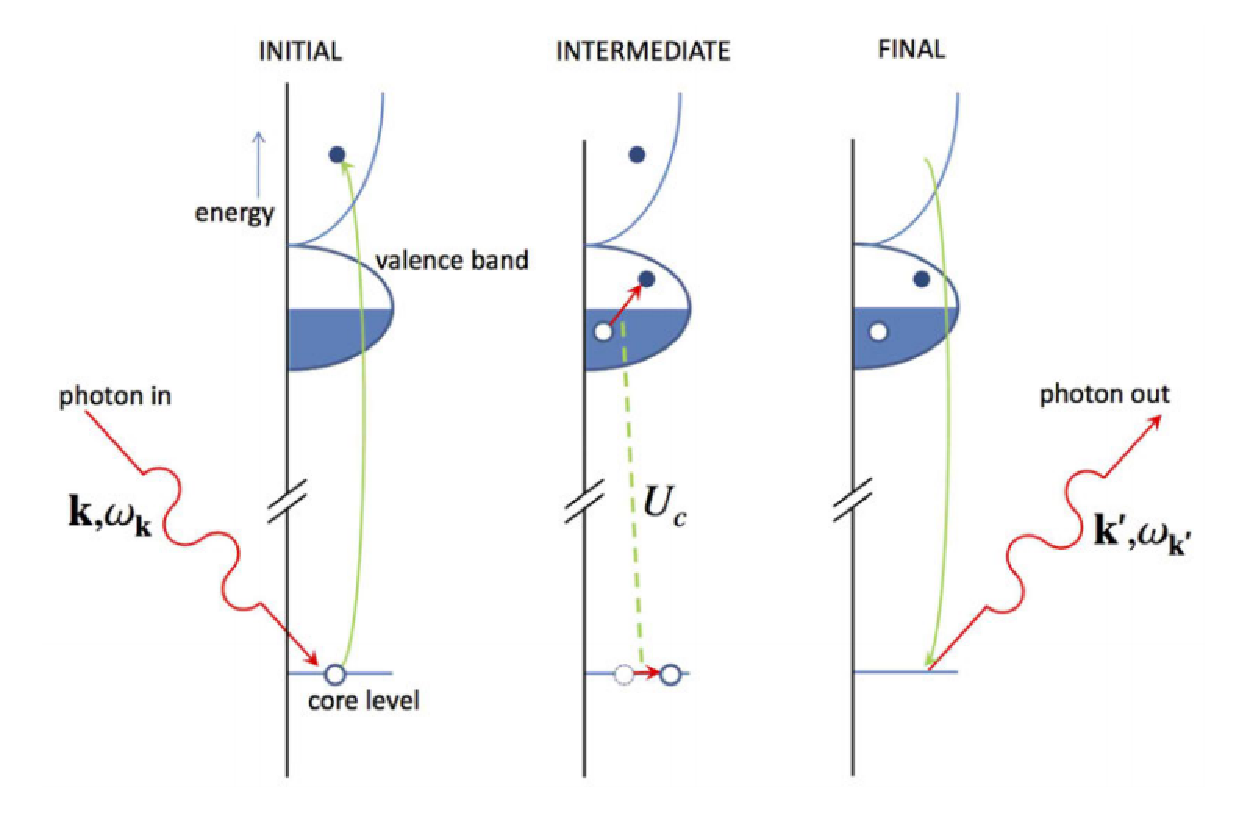
\includegraphics[width=\columnwidth]{Graphics/RIXSprocess.pdf}
	\caption{Typical RIXS process involving creaion of a hole in the valence shell due to core hole-electron coulomb interaction \cite{GuarisePhD} (Pciture taken from \cite{GuarisePhD})}
	\label{fig: RIXSprocess}
    \end{minipage}
   % \hfill
\end{figure}
%---------------------------------------------------------------------------------------------------------------------
\section{Polarization}

%---------------------------------------------------------------------------------------------------------------------
\section{RIXS spectra}

%---------------------------------------------------------------------------------------------------------------------
\section{X-ray Absorption Spectroscopy}
As mentioned before RISX can be essentially seperated into x-ray absorption (XAS) and x-ray photoemission spectroscopy (XPS) with some intermediate interaction described by the green's function of the Kramers-Heisenberg Hamiltonian. The XAS spectrum is directly proprtional to the absorption of the crystal which gives information on magnetic properties of the material. The difference in the absorption using left- and right-cirular polarized x-rays in claed circular magnetic x-ray dichroism (CMXD) ( the similiar differnec in linear polarized light is called LMXD). In order to obtain the CMXD one needs to preserve only the relevant resonances at the copper $L_3$ and $L_2$ edges, which means one needs to model and substract the background assossiated with the excitation of the core electrons into the continuum. The way to do so is to use user-defined bakground function (using for example the arcus tangent) or using the shirley algorithm \cite{Gomez,Shirley}, this is shown in the Fig. S2.
\begin{figure*}
    \begin{minipage}[bp!]{\columnwidth}
        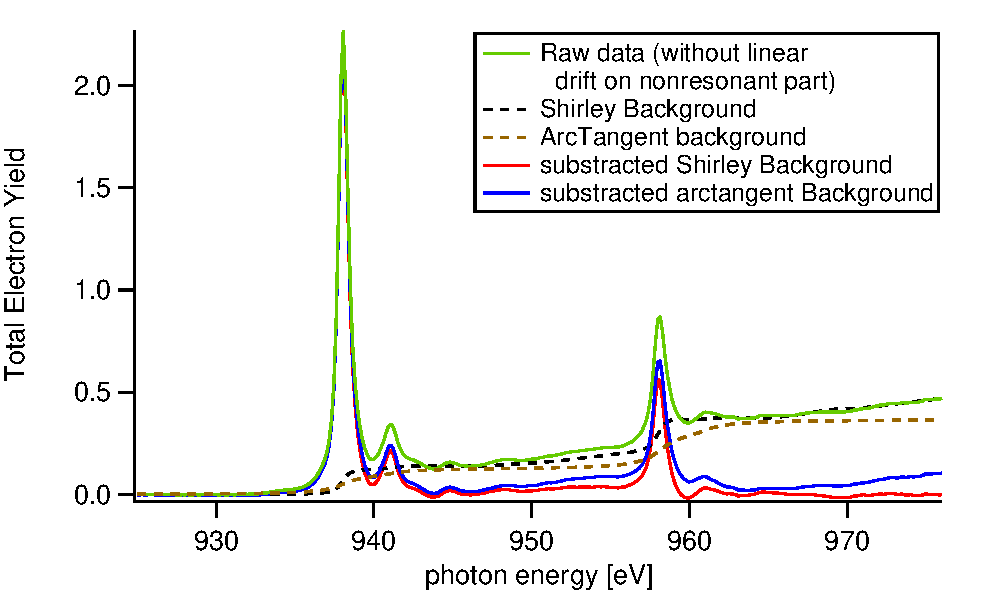
\includegraphics[width=\textwidth]{Graphics/ShirleyBack.pdf}
        \caption{Absorption spectra and modelled background with two different methods}
        \label{fig2}
    \end{minipage}
    \hfil
	\begin{minipage}[bp!]{\columnwidth}
        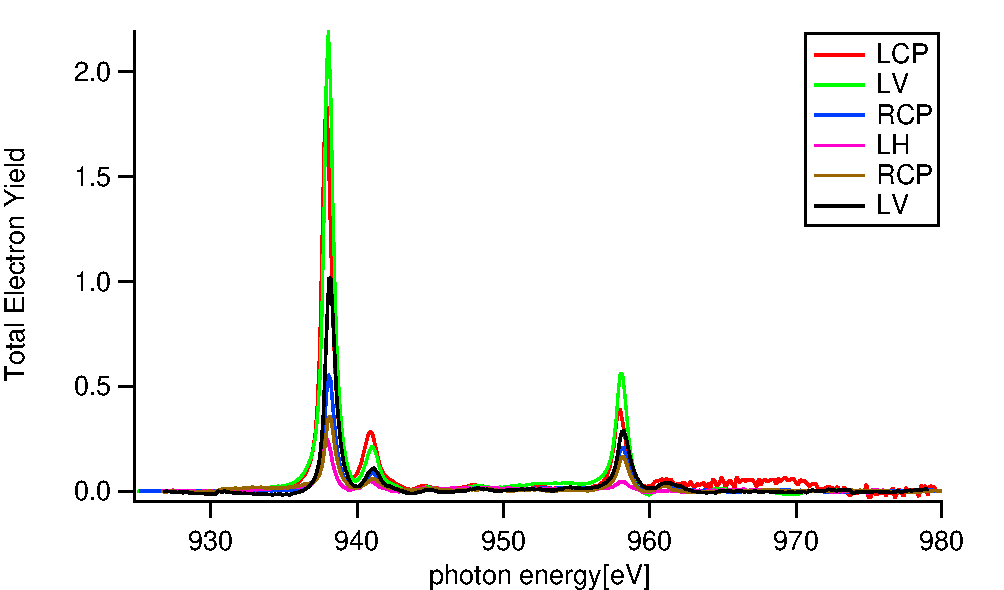
\includegraphics[width=\textwidth]{Graphics/TEY.pdf}
        \caption{Absorption spectra and modelled background with two different methods}
        \label{fig2}
    \end{minipage}l
\end{figure*}
One directly notice that the Shirley algorithm is fitting the backgound much better. Thus for different polarizations this method was used and the corresponing aborption spectra ar drawn in Fig.S3. Now one can proceed to evaluate the CMXD and LMXD on the copper L edges

As was stated by Haverkort \cite{Haverkort} one can use the absorption spectra and their corresponding polarizations to evaluate the conductivity tensor. First of all it is needed to use symmetries to break down the form of the tensor. The relation mentioned in \cite{Haverkort} is

%---------------------------------------------------------------------------------------------------------------------
\section{Results}

\begin{table}
\caption{Example table}
\centering
\begin{tabular}{llr}
\toprule
\multicolumn{2}{c}{Name} \\
\cmidrule(r){1-2}
First name & Last Name & Grade \\
\midrule
John & Doe & $7.5$ \\
Richard & Miles & $2$ \\
\bottomrule
\end{tabular}
\end{table}

\blindtext % Dummy text

\begin{equation}
\label{eq:emc}
e = mc^2
\end{equation}

\blindtext % Dummy text

%------------------------------------------------

\section{Discussion}

\subsection{Subsection One}

A statement requiring citation.
\blindtext % Dummy text

\subsection{Subsection Two}

\blindtext % Dummy text

%----------------------------------------------------------------------------------------
%	REFERENCE LIST
%----------------------------------------------------------------------------------------

\begin{thebibliography}{99} % Bibliography - this is intentionally simple in this template
\expandafter\ifx\csname natexlab\endcsname\relax\def\natexlab#1{#1}\fi
\expandafter\ifx\csname bibnamefont\endcsname\relax
  \def\bibnamefont#1{#1}\fi
\expandafter\ifx\csname bibfnamefont\endcsname\relax
  \def\bibfnamefont#1{#1}\fi
\expandafter\ifx\csname citenamefont\endcsname\relax
  \def\citenamefont#1{#1}\fi
\expandafter\ifx\csname url\endcsname\relax
  \def\url#1{\texttt{#1}}\fi
\expandafter\ifx\csname urlprefix\endcsname\relax\def\urlprefix{URL }\fi
\providecommand{\bibinfo}[2]{#2}
\providecommand{\eprint}[2][]{\url{#2}}
 
\bibitem{Schulke}
W. Sch\"{u}lke,
\textit{Electron dynamics by inelastic x-ray scattering},
Oxford University Press, New York, N.Y., (2007).

\bibitem{Ament2009}
L. J. P. Ament, G. Ghiringhelli, M. M. Sala, L. Braicovich and J. van den Brink
\textit{Theoretical demonstration of how the dispersion of magnetic excitations in cuprate compounds can be determined using resonant inelastic x-ray scattering},
Phys. Rev. Lett. {\bf103}, 117003 (2009).

\bibitem{GuarisePhD}
M. Guarise,
\textit{Electronic and magnetic resonant inelastic x-ray study of cuprates},
PhD-Thesis, EPFL (2012).

\bibitem{Gomez}
A. Herrera-Gomez, M. Bravo-Sanchez, O. Ceballos-Sancheza and M. O. Vazquez-Lepe
\textit{Practical methods for background subtraction in photoemission spectra},
Surf. Interface Anal. 2014, 46, 897–905

\bibitem{Shirley}
D.A. Shirley
\textit{High-Resolution X-Ray Photoemission Spectrum of the Valence Bands of Gold},
Phys. Rev. B 5, 4709 – Published 15 June 1972

\bibitem{Haverkort}
M.W. Haverkort
\textit{Theory of Resonant Inelastic X-Ray Scattering by Collective Magnetic Excitations},
PRL 105, 167404 (2010)

\end{thebibliography}

%----------------------------------------------------------------------------------------

\end{document}
